\documentclass[12pt]{beamer}
%\usetheme{Singapore}
\usecolortheme{ietf91color}

\mode<presentation>
\title{IS-IS Dst/Src Routing \\ \& Critical SubTLVs}
\subtitle{%
  \href{https://datatracker.ietf.org/doc/draft-lamparter-isis-reachability-critical-subtlvs/}{draft-lamparter-isis-reachability-critical-subtlvs-00}\\%
  \href{https://datatracker.ietf.org/doc/draft-baker-ipv6-isis-dst-src-routing/}{draft-baker-ipv6-isis-dst-src-routing-02}
}
\author{%
	Fred Baker $\cdot$ \href{mailto:fred@cisco.com}{fred@cisco.com}\\%
  \underline{David Lamparter $\cdot$ \href{mailto:david@netdef.org}{david@netdef.org}}%
}
\date{IETF 91, Honolulu, Nov. 2014}
\begin{document}

\begin{frame}
  \titlepage
\end{frame}

\begin{frame}
  \frametitle{Context}
  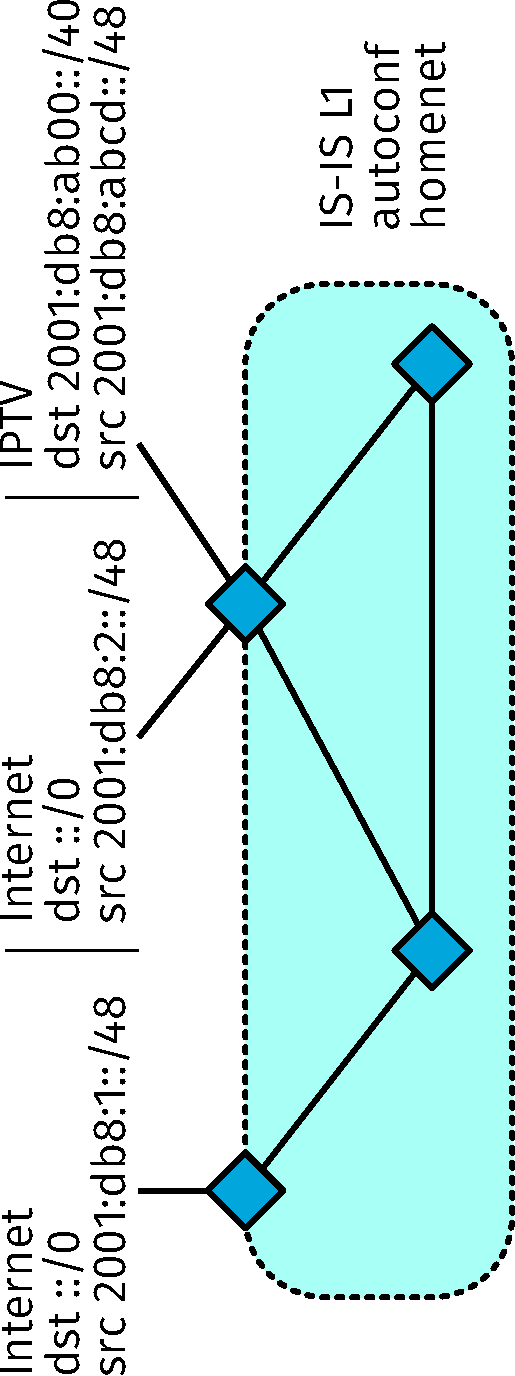
\includegraphics[scale=0.45,angle=-90]{intro_topo.pdf}%
  \vspace{3mm}
  \begin{itemize}
    \item ensuring correct exit taken based on packet source address
    \item BCP 38 ingress filtering at ISP not to be touched
    \item MPTCP needs multiple paths visible at the host
    \item application beyond homenet expected (e.g. SMB)
  \end{itemize}
\end{frame}

\begin{frame}
  \frametitle{NOT-Context}
  This is \textbf{not} MT / Policy routing with a topology per source prefix.

  The expectation is $>95$\% dst routes representing prefixes inside the
  domain, plus $<5$\% dst-src routes representing specific external services.

  All routes go into \textbf{one FIB} which behaves as described in
  \href{https://datatracker.ietf.org/doc/draft-lamparter-rtgwg-dst-src-routing/}{draft-lamparter-rtgwg-dst-src-routing}
\end{frame}

\begin{frame}
  \frametitle{Dst/Src routing is easy}
  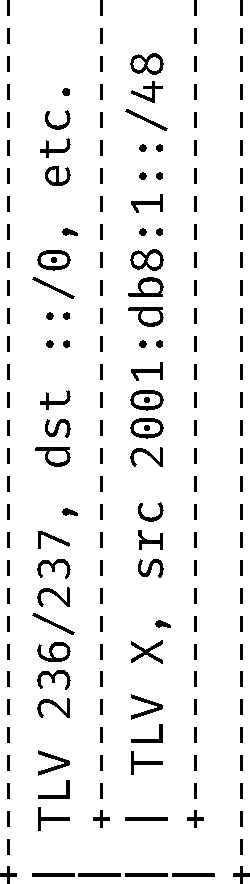
\includegraphics[scale=0.45,angle=-90]{isis_dstsrc_tlv.pdf}%
  \vspace{6mm}
  \begin{itemize}
    \item this is \href{https://datatracker.ietf.org/doc/draft-baker-ipv6-isis-dst-src-routing/}{draft-baker-ipv6-isis-dst-src-routing-02}
    \item sticking the source prefix in is straightforward
    \begin{itemize}
      \item (previous versions forgot to mention MT, that's fixed)
    \end{itemize}
    \item implemented, tested, demo'd @ IETF 90
    \item open source: \url{https://git-us.netdef.org/projects/OSR/repos/openwrt-isis-hnet}
    \item no changes at all to IS-IS ``core''
  \end{itemize}
\end{frame}

\begin{frame}
  \frametitle{Interop is hard}
  \begin{itemize}
    \item naively mixing dst-src routers and non-dst-src routers leads to persistent loops
    \item might be out of scope for homenet
    \item certainly in scope for SMB \& Campus applications
  \end{itemize}
  \vspace{10mm}
  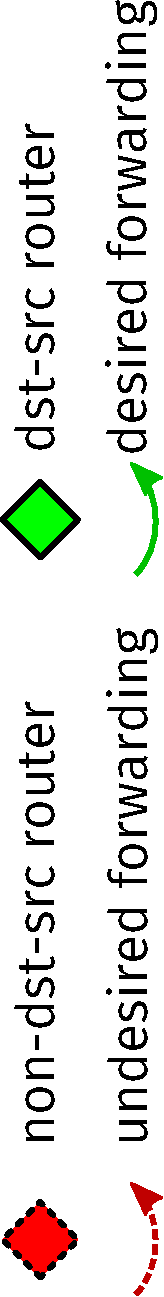
\includegraphics[scale=0.45,angle=-90]{isis_loop_legend.pdf}%
\end{frame}

\begin{frame}
  \frametitle{Loop case \#1}
  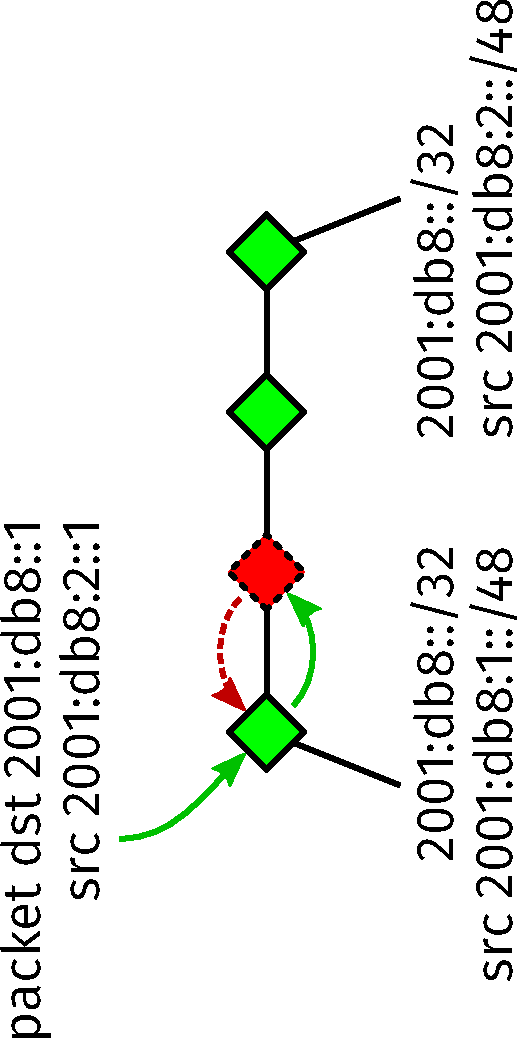
\includegraphics[scale=0.45,angle=-90]{isis_loop1.pdf}%
  \vspace{10mm}
  \begin{itemize}
    \item a dst-src route MUST NOT traverse via a non-dst-src nexthop
  \end{itemize}
\end{frame}

\begin{frame}
  \frametitle{Loop case \#2}
  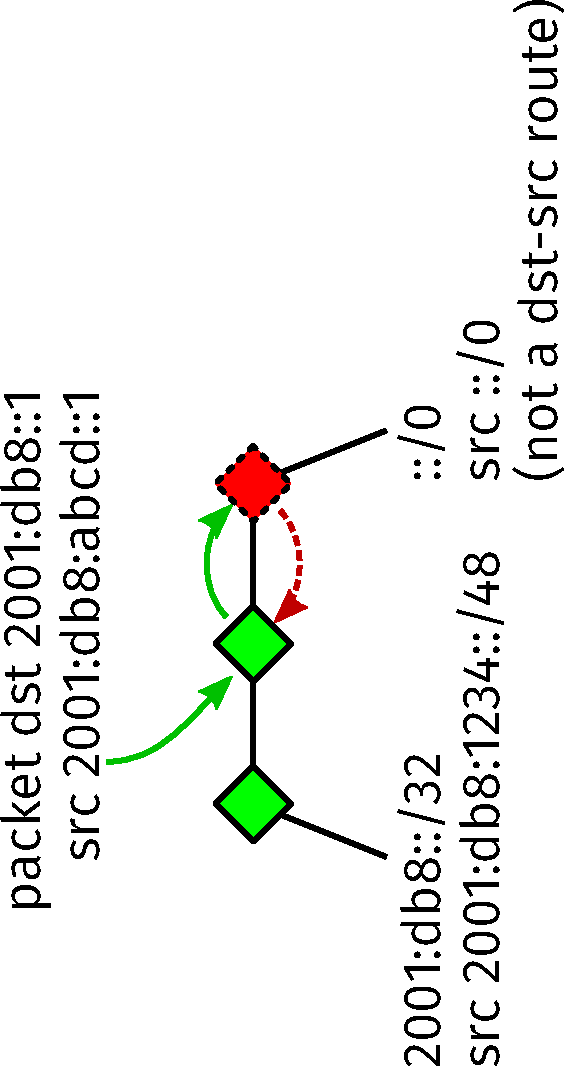
\includegraphics[scale=0.45,angle=-90]{isis_loop2.pdf}%
  \vspace{10mm}
  \begin{itemize}
    \item dst-src routes MUST be ignored by non-dst-src routers
  \end{itemize}
\end{frame}

\begin{frame}
  \frametitle{What do we need}
  To fix these scenarios, we need:
  \begin{itemize}
    \item to fix loop \#1: capability indication
    \item to fix loop \#2: hiding reachabilities from ``old'' systems
  \end{itemize}
  \vspace{5mm}
  The goal is correctness, which can imply blackholing traffic (e.g. if there
  are two islands of dst-src.)  Multiple approaches are possible:
  \begin{itemize}
    \item ``try hard'':\\\hspace{10mm}calculate a separate topology of only dst-src routers
    \item ``fail quick'':\\\hspace{10mm}blackhole when dst-only routers on shortest path
    \item ``fail completely'':\\\hspace{10mm}don't become adjacent with dst-only routers
  \end{itemize}
\end{frame}

\begin{frame}
  \frametitle{Solution attempts}
  Critical Sub-TLV: ``greenfield''/``nice'' solution
  \begin{itemize}
    \item creates new IP Reachability TLVs
    \item has 2 kinds of Sub-TLVs:
    \begin{itemize}
      \item plain optional Sub-TLVs (share a codepoint namespace)
      \item mandatory/critical Sub-TLVs (entire reachability MUST be ignored
        if Sub-TLV is not understood)
    \end{itemize}
    \item implies separate topology/MT based on capabilities\\(in this case:
      separate topology containing only dst-src routers)
  \end{itemize}
  Draft includes a simple capability advertisement mechanism (too simple?)
\end{frame}

\begin{frame}
  \frametitle{Solution attempts}
  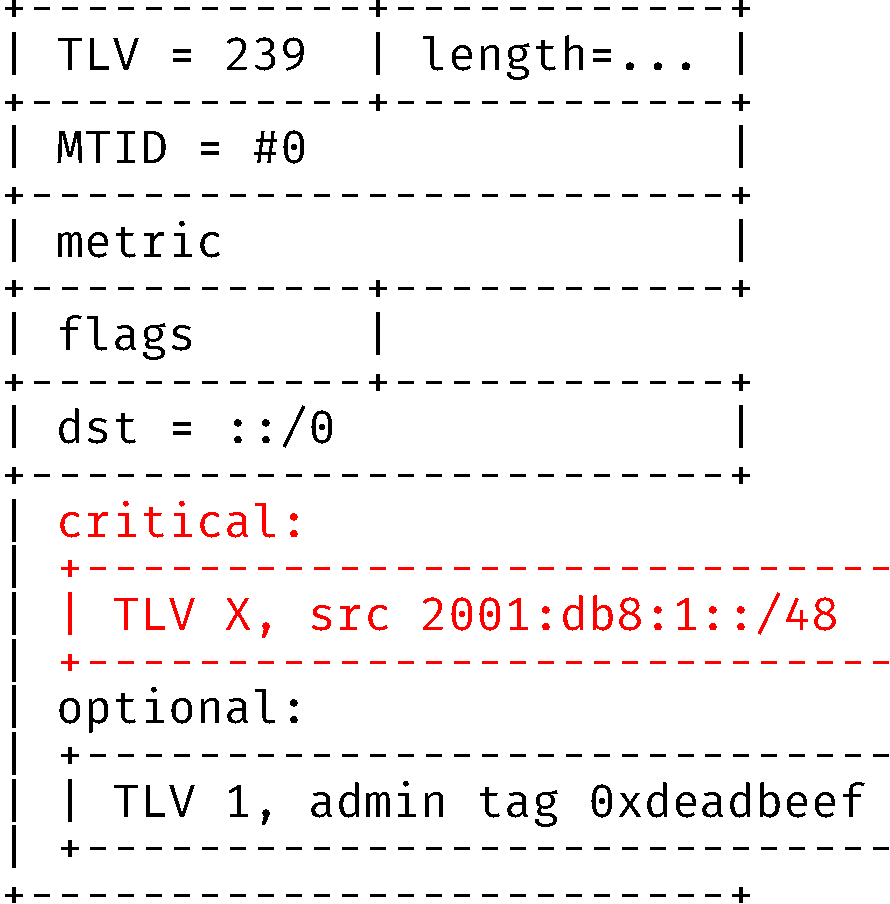
\includegraphics[scale=0.45,angle=0]{isis_dstsrc_subtlv.pdf}%
\end{frame}

\begin{frame}
  \frametitle{Alternative solutions}
  (a) register MTID for dst-src usage
  \begin{itemize}
    \item probably include capability mechanism to prevent dst-src/non-dst-src
       mixture in this particular topology\\
       (to prevent operator self-foot-shooting)
    \item results in 2 MTIDs installed in 1 FIB
  \end{itemize}
  \begin{center}
    -or-\\[3mm]
  \end{center}
  (b) create dst+src main TLV type
  \begin{itemize}
    \item crude way to hide dst-src routes from non-dst-src routers, still
      needs capability indication
  \end{itemize}
\end{frame}

\begin{frame}
  \frametitle{Further path?}
  \begin{itemize}
    \item need to clear topic and proceed
    \item code is running (w/o interop)
  \end{itemize}
\end{frame}

\end{document}
